\documentclass{article}


\usepackage{graphicx}
\usepackage{float}



\title{TNIK Project}
\date{2022-02-22}
\author{Xiangyu Jia}

\begin{document}
\pagenumbering{gobble}
\maketitle
\newpage
\pagenumbering{arabic}

\section{Introduction}
Colorectal cancer (CRC) is a tumor of the digestive system, which has a high incidence, a short survival, 
and a high degree of maligancy, leading to approximately 700 000 deaths worldwide each year. Despite the rapid development of
surgical techniques, the surgical cure rates and 5-year survival rates still remain unsatisfactory. This is due to the high rates
of distant metastasis and postsurgical recurrence. Studies have shown that the majority of CRC patients carry mutations in one 
of two genes invovled in the Wnt/$\beta$-catenin signaling pathways: the adenomatous polyposis coli (APC) and $\beta$-catenin 
(CTNNB1) genes. Among them, more than 80\% show APC mutations; APC is considered a tumor suppressor gene. Mutations in the APC gene
 may cause $\beta$-catenin to fail to degrade and then accumulate in the cytoplasm. Eventually, this surplus $\beta$-catenin 
 translocases to the nucleus as a coactivator of the T-cell fator (TCF)/lymphoid enhancer factor (LEF) family of transcription 
 factors. The accumulated $\beta$-catenin often causes aberrant activation of the T-cell factor 4 (TCF4), a member of the TCF/LEF 
 family of transcription factors, which is a major cause of colorectal carcinogenesis. TNIK (Traf2- and Nck-interacting kinase), is 
 a serine/threonine kinase, is a downstream signal protein in the Wnt/$\beta$-catenin pathway and an ensential regulatory component 
 of the TCF4 and $\beta$-catenin transcription complex. Numerous studies have shown than TNIK could be a suitable target for the 
 treatment of CRC.

\begin{figure}[h]
  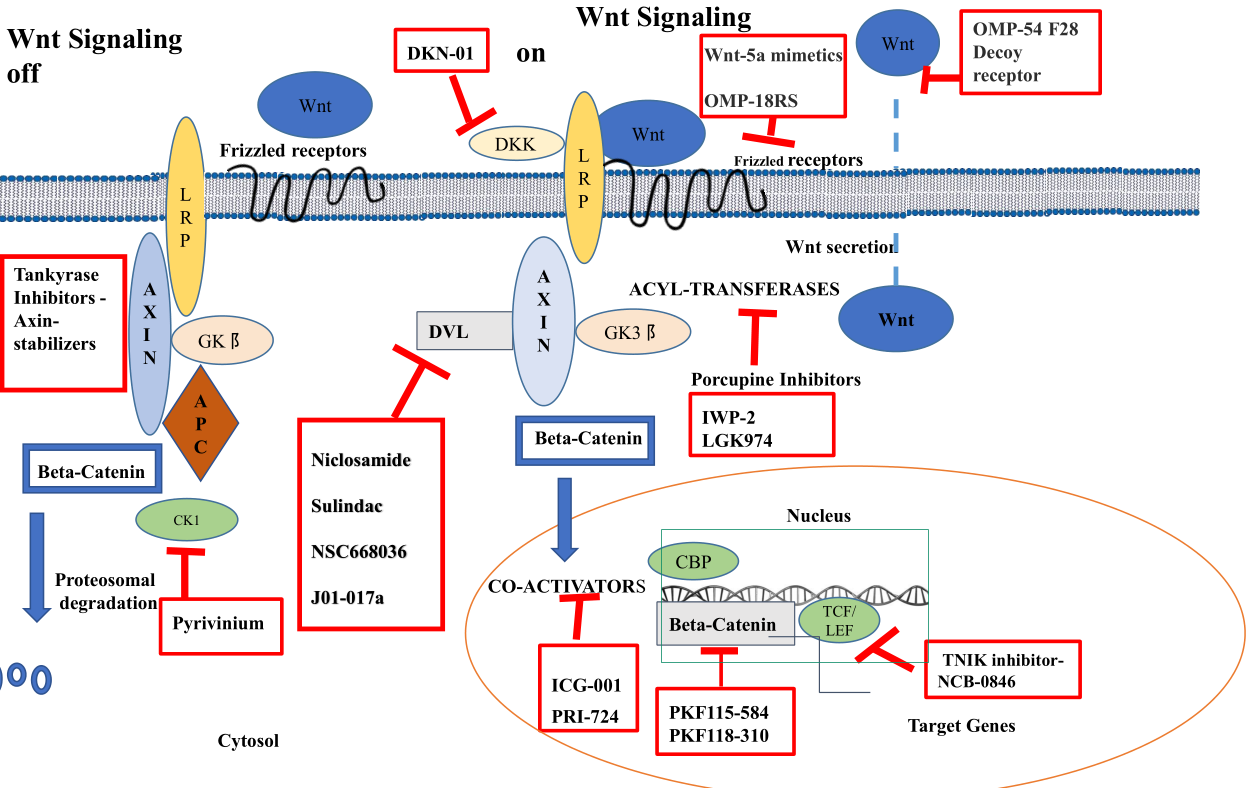
\includegraphics[width=\linewidth]{pathway.png}
  \caption{Canonical Wnt Pathway and Inhibitors of the Wnt/$\beta$-Catenin Signaling Pathwat}
  \label{pathway}
\end{figure}


\section{Some previous studies}
\subsection{ACS Comb.sci. 2020,22,608-616}

\end{document}